\chapter{Modelado de sistemas dinámicos}\label{modelado}

\section{Sistemas en el espacio de estados}
Nos vamos a centrar en sistemas que puedan ser descritos por características cuantificables. A estas características las vamos a llamar {\bf variables de estado}, como por ejemplo, una temperatura, una velocidad, o un voltaje. Si estas variables de estado dependen del tiempo, entonces, llamamos {\bf señal} a la sucesión de valores de las variables de estado en el tiempo. Uno podría interaccionar con el sistema a través de una {\bf entrada} cuantificable, y a su vez medir información del sistema a través de una {\bf salida} cuantificable.

Vamos a definir $x(t)\in\mathbb{R}^n$, $y(t)\in\mathbb{R}^m$ y $u(t)\in\mathbb{R}^k$ respectivamente, como el vector apilado de variables estados, la salida, y la entrada a un sistema $\Sigma$. En particular, variables de estado, entradas y salidas son señales, e.g., $x :[0,\infty) \to \mathbb{R}^n$.

El sistema $\Sigma$ es un modelo que predice el valor de las variables de estado y la salida a lo largo del tiempo. Esta predicción incorpora la interacción de la entrada con los estados y la salida. En particular, vamos a emplear ecuaciones diferenciales como herramienta para predecir la evolución en el tiempo de los estados del sistema $\Sigma$ como se muestra a continuación
\begin{equation}
	\Sigma := \begin{cases}
		\dot x(t) =& f(t,x(t),u(t)) \\ y(t) =& g(t,x(t),u(t))
	\end{cases}, 
\label{eq: sigma}
\end{equation}
en donde $\dot x := \frac{\mathrm{d}}{\mathrm{dt}}(x(t))$ es la notación para la derivada total con respecto del tiempo, y $f:\mathbb{R} \times \mathbb{R}^n \times \mathbb{R}^k \to \mathbb{R}^n$ y $g: \mathbb{R} \times \mathbb{R}^n \times \mathbb{R}^k \to \mathbb{R}^m$ son funciones.

Podemos representar el sistema $\Sigma$ como un bloque con puertos de entrada y de salida como se muestra en la figura \ref{fig: sigma}.

\begin{figure}[!ht]
\centering
\begin{tikzpicture}[auto, node distance=2cm,>=latex']
	\node [input, name=input] {};
	\node [block, right of=input] (system) {$\Sigma$};
	\node [output, right of=system] (output) {};
	\draw [draw,->] (input) -- node {$u(t)$} (system);
	\draw [->] (system) -- node [name=y] {$y(t)$}(output);
\end{tikzpicture}
	\caption{Diagrama de bloque entrada/salida del sistema $\Sigma$.}
	\label{fig: sigma}
\end{figure}

Dado que el sistema viene descrito por las variables de estado,  con frecuencia es posible prescindir de la salida y centrar el estudio en la primera de las dos ecuaciones anteriores.

 En ocasiones podemos emplear para describir un sistema ecuaciones de estado en las que no aparece explícitamente la entrada,
\begin{equation}
\dot x = f(t,x)
\end{equation}\label{eq: for}
En este caso, se habla de una ecuación de estado no forzada. Esto no quiere decir necesariamente que la entrada al sistema sea cero. Puede aparecer representada directamente como una función del tiempo, $u=\rho(t)$,  como una función (\emph{realimentación}) de los estados $u = \rho(x)$ o como una función de ambos $u=\rho(t,x)$.
Un caso especialmente interesante de (\ref{eq: for}) se obtiene cuando $f$ no depende explícitamente del tiempo,
\begin{equation}
\dot x = f(x)
\end{equation}
Se trata entonces de un sistema \emph{autónomo} o \emph{invariante en el tiempo}. Es decir, el comportamiento del sistema es invariante bajo traslaciones del origen de tiempos; si cambiamos la variable tiempo de $t$ a $t-a$, la parte derecha de la ecuación de estado no experimenta cambio.

Para un sistema dinámico, descrito mediante variable de estados, un punto de equilibrio $\overline x$  tiene la propiedad de que si el sistema se encuentra en $\overline x$ en un instante de tiempo $t_0$, permanecerá en ese  mismo punto para todo instante de tiempo posterior $t>t_0$. En el caso de un sistema autónomo, los puntos de equilibrio son las raíces reales de la ecuación,
\begin{equation}
f(x)=0
\end{equation} 

Los puntos de equilibrio juegan un papel muy importante en el estudio de los sistemas dinámicos, como tendremos ocasión de ver más adelante.

Un caso particular de sistema dinámicos los constituyen los sistemas lineales. Para ellos la ecuación \ref{eq: sigma} toma la forma,
\begin{equation}
	\Sigma := \begin{cases}
		\dot x(t) =& A(t)x(t)+B(t)u(t) \\ y(t) =& C(t)x(t)+D(t)u(t)
	\end{cases}, 
\label{eq: sigmaL}
\end{equation}

En el capítulo 5 se estudiarán en detalle los sistemas lineales, cuyas propiedades permiten emplear herramientas de análisis precisas y potentes para su estudio y caracterización. En el caso del resto de los sistemas, es decir todos aquellos que son no-lineales, el análisis resulta más complejo.

Una primera aproximación al estudio de los sistemas no-lineales es linealizarlos en torno a un punto de trabajo y estudiar el sistema lineal resultante. Esta aproximación es muy valiosa, como  veremos en la sección (\ref{sec: linear}), sin embargo, solo es válida en las proximidades del punto de trabajo. Por tanto no es posible predecir a partir de ella el comportamiento del sistema cuando nos alejamos de dicho punto. Por otro lado, los sistemas no-lineales presentan una dinámica mucho mas rica, con fenómenos que no se dan en los sistemas lineales y que no pueden describirse con un modelo linealizado del sistema no-lineal. Algunos de éstos fenómenos son:

\paragraph{Múltiples puntos de equilibrio aislados.} Para un sistema lineal solo es posible encontrar un punto de equilibrio o una región continua de ellos (rectas, planos, etc).  Un sistema lineal es asintóticamente estable cuando, partiendo de valores iniciales arbitrarios, sus variables de estado se aproximan al punto de equilibrio con el tiempo. 

\begin{equation}
\lim_{ t \to \infty} x \to \overline x
\end{equation}


Un sistema no lineal puede presentar más de un punto de equilibrio y aproximarse a uno u otro dependiendo de las condiciones iniciales.

\paragraph{Tiempo de escape finito (\emph{Finite escape time}).} Un sistema lineal es inestable cuando, partiendo de valores arbitrarios, sus variables de estado divergen --se van a infinito-- con el tiempo.
\begin{equation}
\lim_{ t \to \infty} x \to \infty
\end{equation}
Es posible encontrar sistemas no-lineales inestables que se comportan de modo análogo a los lineales pero además, algunos sistemas no lineales divergen, se van a infinito, en un tiempo finito. 
\begin{equation}
\lim_{ t \to t_e} x \to \infty
\end{equation}

\paragraph{ciclos límite.} Un sistema lineal se dice que es marginalmente estable, cuando sus variables de estado oscilan periódicamente. Sin embargo, como veremos más adelante, las circunstancias para que se de una oscilación mantenida en un sistema lineal, constituyen una condición no robusta, por lo que es en la práctica  imposible que se dé en condiciones reales. Además, la amplitud de las oscilaciones depende de las condiciones iniciales del sistema.

Hay sistemas no lineales que pueden oscilar de modo estable con una amplitud y frecuencia independiente de las condiciones iniciales. A este tipo de oscilaciones se les conoce con el nombre de ciclos límite. 

\paragraph{Caos.} Algunos sistemas no-lineales exhiben comportamientos aún más complicados. No alcanzan un punto de equilibrio, no presentan oscilaciones periódicas, ni tampoco son inestable. A este comportamiento se le denomina caótico. Alguno sistemas presentan incluso un comportamiento aleatorio, a pesar de la naturaleza determinista de las ecuaciones diferenciales que lo definen.


 Resulta por tanto necesario, buscar herramientas específicas para el análisis de los sistemas no-lineales.
\section{Ejemplos de sistemas dinámicos}\label{sec: ejem}
A continuación se presentan algunos ejemplos clásicos de sistemas dinámicos.
\begin{example}[Péndulo invertido]

Vamos a derivar las funciones $f$ y $g$ en (\ref{eq: sigma}) para el sistema del péndulo invertido.

Primero, vamos a hallar la ecuación diferencial que describe la dinámica de una masa $m\in\mathbb{R}_+$ en el extremo de un péndulo de longitud $l\in\mathbb{R}_+$ tal y como se muestra en la figura \ref{fig: invpen}. Vamos a considerar que podemos interactuar con el sistema por medio de un torque $T\in\mathbb{R}$ en el otro extremo del péndulo, que la masa sufre un rozamiento proporcional $b\in\mathbb{R}_+$ a su celeridad, y que podemos medir el ángulo $\theta\in\mathbb{R}$ que forma el péndulo con la vertical.

\begin{figure}[!ht]
\centering
\begin{tikzpicture}
    \coordinate (origo) at (0,0);
    \coordinate (pivot) at (1,5);

    % draw axes
	\fill[black] (origo) circle (0.05) ++ (-0.25,0.25) node (T) [black] {$T$} ++(0.75,0.75) node (l) [above] {$l$};
    \draw[thick,gray,->] (origo) -- ++(4,0) node[black,right] {$x$};
    \draw[thick,gray,->] (origo) -- ++(0,4) node (mary) [black,above] {$y$};

    % draw roof
    \fill[pattern = north east lines] ($ (origo) + (-1,0) $) rectangle ($ (origo) + (1,-0.5) $);
    \draw[thick] ($ (origo) + (-1,0) $) -- ($ (origo) + (1,0) $);

    \draw[thick] (origo) -- ++(-300:3) coordinate (bob) ++(0.5,0) node (hola) [black] {$m$};
    \fill (bob) circle (0.2);
    \draw[->] (bob) -- ++(0,-1) node (mg) [right] {$mg$};
    \draw[->] (bob) -- ++(-0.5,0.5) node (fr) [above] {$b\dot\theta$};

    \pic [draw, <-, "$\theta$", angle eccentricity=1.5] {angle = bob--origo--mary};
\end{tikzpicture}
\caption{Péndulo Invertido}
\label{fig: invpen}
\end{figure}

Define $g = 9.8$ e $I\in\mathbb{R}_+$ como la aceleración gravitatoria y el momento de inercia del péndulo respectivamente. Es sencillo comprobar que $I = ml^2$, y explotaremos que $I \ddot\theta = \text{suma de torques}$. De hecho, tenemos que considerar tres torques: 1. Torque $T$ ejercido por nosotros en la base del péndulo; 2. Torque $-bl\dot\theta$ ejercido por la fricción en la masa; 3. Torque $mgl \sin\theta$ ejercido por la atracción gravitatoria. Por lo que la ecuación diferencial que modela el comportamiento del péndulo invertido es
\begin{equation}
\ddot\theta = \frac{1}{ml^2}\left(mgl\sin{\theta}-bl\dot\theta + T\right).
\label{eq: dyn}
\end{equation}

Parece razonable escoger $\theta$ como uno de los estados para construir $x(t)$ en (\ref{eq: sigma}). De hecho, la ecuación (\ref{eq: dyn}) es de segundo orden en $\theta$, por lo que es conveniente escoger $\dot\theta$ como un estado también. Por lo tanto, definamos nuestro vector de estados como
\begin{equation}
x := \begin{bmatrix}\theta \\ \dot\theta \end{bmatrix},
\end{equation}
y dado que mediante el torque $T$ es como interactuamos con el sistema, escogemos como entrada $u(t) = T(t)$.

Ahora estamos listos para construir las funciones $f$ and $g$ en (\ref{eq: sigma}) para el péndulo invertido. Atención a que $f$ y $g$ solo toma como argumentos los vectores de estados $x$ y de entradas $u$. En el lado izquierdo de (\ref{eq: sigma}) tenemos la derivada temporal de $x(t)$, por lo que

\begin{equation}
	\frac{\mathrm{d}}{\mathrm{dt}}\left(\begin{bmatrix}\theta \\ \dot\theta \end{bmatrix}\right) = f(x(t), u(t)) = \begin{bmatrix}f_1(x(t), u(t)) \\ f_2(x(t), u(t))\end{bmatrix}, \label{eq: fn}
\end{equation}
donde automáticamente obtenemos que $f_1 = \dot\theta$. Fijarse que la primera fila de $f$ en (\ref{eq: fn}), a la izquierda tenemos que $\frac{\mathrm{d}}{\mathrm{dt}}\theta$, y a la derecha tenemos que $f_1 = \dot\theta$ porque $\dot\theta$ es un estado o elemento de $x$. Desafortunadamente, no podemos decir que $f_2 = \ddot\theta(t)$ porque $ \ddot\theta$ no es un estado o elemento de $x$. No obstante, tenemos que la segunda fila $f_2$ viene dada por la ecuación (\ref{eq: dyn}). Por lo que podemos escribir $f$ como
\begin{equation}
	\frac{\mathrm{d}}{\mathrm{dt}}\left(\begin{bmatrix}\theta \\ \dot\theta \end{bmatrix}\right) =  f(x(t), u(t)) = \begin{bmatrix} \dot\theta \\ \frac{1}{ml^2}\left(mgl\sin{\theta}-bl\dot\theta + T\right) \end{bmatrix}. \label{eq: f}
\end{equation}

El cálculo de $g$ es más sencillo en este caso. Hemos establecido al comienzo que solo podemos medir el ángulo $\theta$. Por lo que $y(t) = \theta(t)$, i.e.,
\begin{equation}
g(x(t),u(t)) =  \theta(t).
	\label{eq: g}
\end{equation}

%A Python simulation of this dynamics can be found at \url{https://github.com/noether/aut_course}.
\qed 
\end{example}

\begin{example}[El oscilador de Van der Pol]
Se trata de un oscilador, propuesto por primera vez por Balthasar Van der Pol, cuando trabajaba en Philips, para explicar las oscilaciones observadas en tubos de vacío. Podemos obtener la ecuación del oscilador, empleando el circuito de la figura \ref{fig:vdp}.
\begin{figure}
\centering
\begin{circuitikz}[american, scale = 0.6]\draw
(0,-4)to[short]
(4,-4)to[short,,i^<= $i_C$]
(5,-4)to[short,i=$i_N$]
(6,-4)to[short](10,-4)
(0,-7.5)to[C = C](0,-4)
(5,-4) to[L = L, i>^= $i_L$,*-* ](5,-7.5)
(10,-4) to[generic=NL,  i= $i_N \equiv h(v)$](10,-7.5) 
(0,-7.5)to[short](10,-7.5)
;
\end{circuitikz}
\caption{Circuito eléctrico no lineal}
\label{fig:vdp}
\end{figure}

Donde el elemento no lineal NL, presenta una relación entre voltaje e intensidad caracterizada por la función $h(v)$.

El voltaje $v$ en los tres componentes del circuito debe ser igual; además,
\begin{align}
v = L \frac{di_L}{dt}\\
i_C = C\frac{dv}{dt}\\
i_N = h(v)
\end{align}
Si aplicamos la primera ley de Kirchohff al nodo superior del circuito,
\begin{align}
i_C+i_L+i_N = 0\\
C\frac{dv}{dt}+\frac{1}{L}\int_{-\infty}^{t}v(s)ds +h(v)=0\label{eq:vdp}
\end{align}
Si derivamos (\ref{eq:vdp}) con respecto al tiempo, dividimos por $C$ y reordenamos,
\begin{equation}\label{eq:vdp2}
\frac{d^2v}{dt^2}  + \frac{1}{C}\frac{dh(v)}{dv}\frac{dv}{dt} + \frac{1}{LC}\cdot v= 0
\end{equation}
Se trata de un caso particular de la ecuación de Liénard,
\begin{equation}
\ddot{v} +f(v)\dot{v}+g(v) = 0
\end{equation}
Si definimos ahora, $h(v)$,
\begin{align}
h(v) = m(\frac{1}{3}v^3-v)\\
\frac{dh}{dv} = m(v^2-1)
\end{align}
y sustituimos en (\ref{eq:vdp2}),
\begin{equation}
\ddot{v} +m\frac{1}{C}(v^2-1)\dot{v}+\frac{1}{LC}v = 0
\end{equation}

Podemos representarla finalmente en variables de estado, tomando $x_1=v$ y $x_2=\dot{v}$,
\begin{align}
\dot{x}_1 &= x_2 \label{eq:vpst1} \\
\dot{x}_2 &= -\frac{1}{LC}x_1 - m\frac{1}{C}(x_1^2-1)x_2 \label{eq:vdpst2}
\end{align}
Podemos ahora hacer un primer análisis cualitativo. El primer término a la derecha del igual en  la ecuación (\ref{eq:vdpst2}) representa una fuerza recuperadora proporcional al desplazamiento, el segundo término, crecerá con la velocidad para $x_1 < 1$, alejando así al sistema del origen  y representará un término disipativo para $x_1 > 1$ acercándolo por tanto de nuevo al origen. Es por tanto esperable, que se alcance
algún tipo de situación de equilibrio. Más adelante definiremos esta situación rigurosamente como un ciclo límite. \qed
\end{example} 
\begin{example}[Un vehículo de cuatro ruedas.]
La figura \ref{fig:vehir} muestra un esquema de un vehículo terrestre de cuatro ruedas, visto desde arriba. Si consideramos que se mueve en el plano $x,y$, y que su velocidad instántanea $\vec{V}$ está siempre orientada en la dirección de avance del vehículo $\psi$ --asumimos que no derrapa, ni se mueve lateralmente--, podemos entonces definir la velocidad, en el sistema de referencia $x,y$ como,
\begin{align}
\dot{x} = V_x(t) = V\cos(\psi(t))\\
\dot{y} = V_y(t) = V\sin(\psi(t)).
\end{align}

\begin{figure}
\centering

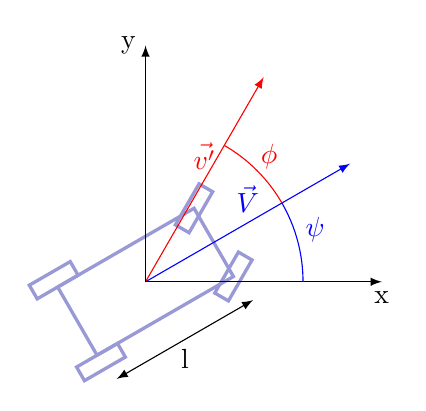
\begin{tikzpicture}
\draw(0,0)[rotate around={30:(0,0)},very thick,draw = blue!60!black!40]rectangle(2,1);
\draw(-0.3,-0.2)[rotate around={30:(0,0)},very thick,draw = blue!60!black!40]rectangle(0.3,0.0);
\draw(-0.3,1)[rotate around={30:(0,0)},very thick,draw = blue!60!black!40]rectangle(0.3,1.2);
\draw({2*cos(30)-0.3},{2*sin(30)-0.1})[rotate around={60:({2*cos(30)},{2*sin(30)})},very thick,draw = blue!60!black!40]rectangle({2*cos(30)+0.3},{2*sin(30)+0.1});
\draw({2*cos(30)-sin(30)-0.3},{2*sin(30)+cos(30)-0.1})[rotate around={60:({2*cos(30)-sin(30)},{2*sin(30)+cos(30)})},very thick,draw = blue!60!black!40]rectangle({2*cos(30)-sin(30)+0.3},{2*sin(30)+cos(30)+0.1});
\draw[blue]({cos(30)-0.5*sin(30)},{sin(30)+0.5*cos(30)})--node[above]{$\vec{V}$}({4*cos(30)-0.5*sin(30)},{4*sin(30)+0.5*cos(30)})[-latex];
\draw[red]({cos(30)-0.5*sin(30)},{sin(30)+0.5*cos(30)})--node[above]{$\vec{v'}$}({cos(30)-0.5*sin(30)+3*cos(60},{sin(30)+0.5*cos(30)+3*sin(60})[-latex];

\draw({cos(30)-0.5*sin(30)},{sin(30)+0.5*cos(30)})--({3+cos(30)-0.5*sin(30)},{sin(30)+0.5*cos(30)})[-latex]node[anchor=north]{x};
\draw({cos(30)-0.5*sin(30)},{sin(30)+0.5*cos(30)})--({cos(30)-0.5*sin(30)},{3+sin(30)+0.5*cos(30)})[-latex]node[anchor=east]{y};

\draw[blue]({2+cos(30)-0.5*sin(30)},{sin(30)+0.5*cos(30)})arc(0:30:2);
\draw[red]({3*cos(30)-0.5*sin(30)},{3*sin(30)+0.5*cos(30)})arc(30:60:2);
\draw[blue]({3.2*cos(30)},{3.2*sin(30)}) node[]{$\psi$};
\draw[red]({3.4*cos(50)},{3.3*sin(50)}) node[]{$\phi$};
\draw[latex-latex](0.25,-0.3)--node[below]{l}({2*cos(30)+0.25},{2*sin(30)-0.3});
\end{tikzpicture}
\caption{Esquema de un vehículo terrestre de 4 ruedas}
\label{fig:vehir}
\end{figure}

Además el vehículo girará, siempre que las ruedas delanteras no estén alineadas con las ruedas traseras, cambiando así su dirección de avance . Podemos relacionar la velocidad de giro del vehículo $\dot{\psi}$ con el ángulo de orientación de las ruedas delanteras $\phi$, y la velocidad a la que avanzan $\vec{v}'$.  podemos obtener las componentes de dicha velocidad en ejes cuerpo (paralela y perpendicular a la dirección de avance del vehículo),

\begin{align}
v_{P} = v'\cos(\phi(t))\\
v_{T} = v'\sin(\phi(t))
\end{align} 

Pero la rueda esta unida al vehículo así que su velocidad en la direccíon de avance debe ser la misma que la del vehículo: $v_P \equiv V$.  A partir de esta relación podemos obtener la velocidad tangencial de las ruedas como,
\begin{equation}
v_T = V\frac{\sin(\phi)}{\cos(\phi)} = V\tan(\phi)
\end{equation}

Si tomamos como centro de giro del vehículo el centro de su eje trasero, y la batalla (distancia entre ejes) es $l$, obtenemos una expresión para su velocidad de giro,
\begin{equation}
\dot{\psi} = \frac{V}{l}\tan(\phi)
\end{equation}

En resumen, podemos describir el sistema mediante tres ecuaciones de estado $x_1 \equiv x, x_2\equiv	y, x_3 \equiv \psi$:

%\begin{align}
%\dot{x}_1 =  V\cos(x_3)\\  
%\dot{x}_2 =  V\sin(x_3)\\
%\dot{x}_3 = \frac{V}{l}\tan(\phi)
%\end{align}

\begin{equation}
	\begin{cases}
		\dot x_1 &=  V\cos(x_3)\\  
		\dot x_2 &=  V\sin(x_3)\\
		\dot x_3 &= \frac{V}{l}\tan(\phi)
	\end{cases}
\end{equation}

Si consideramos $V=cte$, la única entrada al sistema sería el ángulo de giro de las ruedas $u(t) = \phi(t)$, controlando su valor, podemos hacer girar al vehículo en la dirección deseada. \qed
\end{example}

\section{Simulación o soluciones numéricas del sistema $\Sigma$}
Dado un punto inicial $x(0)$, podemos predecir o calcular numéricamente $x(t)$. El método de \emph{integración de Euler} es un método numérico sencillo que puede darnos información sobre la evolución temporal de los estados y salidas de $\Sigma$. El siguiente algoritmo describe la integración numérica por Euler:
\begin{algo}   \ \\
	\begin{enumerate}
		\item Define el paso de tiempo $\Delta T$
		\item Define $x = x(0)$
		\item Define $y = g(x,u)$
		\item Registra $x$ and $y$, para poder procesarlos después si fuera necesario
		\item Define $t = 0$
		\item Define un tiempo final $t^*$
		\item Mientras $t \leq t^*$ entonces:
			\begin{enumerate}
				\item $x_{\text{nuevo}} = x_{\text{viejo}} + f(x_{\text{viejo}},u)\Delta T$
				\item $y_{\text{nuevo}} = g(x_{\text{nuevo}},u)$
				\item Representa $x$ gráficamente
				\item Registra $x$ e $y$, para poder procesarlos más adelante si fuera necesario
				\item $t = t + \Delta t$
			\end{enumerate}
		\item Representa $x$ e $y$ a lo largo de $t$
	\end{enumerate}
\end{algo}

Este algoritmo rinde bien cuando $\Delta T$ es suficientemente pequeño en función de como de rápido varíe $f$ en el tiempo. Por ahora hemos considerado $u=0$, es decir, no hay control o interacción alguna con el sistema.

Existen, métodos más robustos para obtener la solución numérica de un sistema. Entre ellos, destacan los métodos de Runge-Kutta, y en particular, el uso de los llamados 'pares encajados' de dichos métodos. Describir los detalles de cálculo de dichos métodos queda fuera del alcance de estas notas. Hay muchos paquetes de software como Matlab o Python que incluyen funciones que implementan dichos métodos. En  el apéndice \ref{apend1}. Se incluyen códigos de Matlab con ejemplos y explicaciones de como construirlos.

\section{Sistemas autónomos de segundo orden}
Los sistema autónomos de segundo orden, son especialmente atractivos para el estudio de los fenómenos no lineales porque sus soluciones se pueden representar fácilmente en el llamado plano de fases.
En general, podemos definir un sistema autónomo de segundo orden a partir de dos ecuaciones escalares, una para la derivada temporal de cada estado,
\begin{align}
\dot x_1 &= f_1(x_1,x_2) \label{eq: sysa1}\\
\dot x_2 &= f_2(x_1,x_2) \label{eq: sysa2}
\end{align}

Supongamos que conocemos una solución al sistema $x(t) = [x_1(t),x_2(t)]^T$, que pasa por el punto $x(0) = x_0$. La solución describe una curva sobre el plano $x_1-x_2$ que pasa por el punto $x_0$. Esta curva recibe el nombre de trayectoria u órbita, desde $x_0$, del sistema. El plano $x_1-x_2$ recibe el nombre de plano de fases. La ecuaciones (\ref{eq: sysa1}) - (\ref{eq: sysa2}) representan un vector tangente $\dot x(t) = [\dot x_1(t),\dot x_2(t)]$ a la trayectoria en el punto $x(t)$.

Además podemos considerar $f(x)=[f_1(x),f_2(x)]$ como un campo vectorial definido sobre el plano de fases., es decir asignamos a cada punto $x$ en el espacio de fases el vector $f(x)$. Es posible obtener una representación aproximada del campo vectorial asociado a un sistema si definimos una región de interés del plano de fase, por ejemplo, una región que contenga sus puntos de equilibrio. Seleccionamos un conjunto de puntos $x$ en posiciones equiespaciadas dentro de la región de interés, y representamos en cada punto $x$ el campo asociado $f(x)$ mediante una flecha que apunte en la dirección de $f(x)$ y cuya longitud sea proporcional al módulo de $f(x)$.

El conjunto de todas las trayectorias en el plano de fases de un sistema se denomina su diagrama de fases. de modo análogo al caso de campo vectorial, podemos obtener una representación aproximada del diagrama de fases obteniendo las trayectorias del sistemas para un conjunto suficientemente grande de condiciones iniciales en una región de interés y dibujándolas en el plano de fases.

\subsection{Algunos ejemplos}
Las representaciones en el plano de fases, nos ofrecen un camino sencillo para observar algunos de los fenómenos propios de los sistemas no lineales. A continuación, vamos a emplearlas con algunos de los ejemplos de la sección \ref{sec: ejem}
\begin{example}[Diagrama de fases para el péndulo invertido \ref{Apinv}]
Podemos obtener un sistema autónomo para el péndulo invertido, eliminando la tensión $T$ de las ecuaciones \ref{eq: f},
\begin{figure}
\includegraphics[scale=0.8]{resp_p_inv.eps}
\caption{Evolución temporal y trayectoria en el plano de fases para el péndulo invertido. La condición inicial, $x_0=[\pi/3,0]^T$, aparece representada con un aspa en el espacio de fases.} \label{fig:trpen}
\end{figure}

\begin{align}
\dot x_1 = &x_2 \label{eq:pi1} \\ 
\dot x_2 = &\frac{g}{l}\sin x_1 - \frac{b}{ml}x_2 \label{eq:pi2}
\end{align}
donde $x_1 = \theta$ y $x_2 = \dot \theta$,. Una primera característica del sistema la obtenemos calculando los puntos de equilibrio, $\overline x=[n\pi,0]^T, n \in \mathbb{Z}$. Tenemos un conjunto infinito de posibles puntos de equilibrio, correspondiente a las posiciones verticales del péndulo.

La figura \ref{fig:trpen} muestra una trayectoria del péndulo invertido para una realización particular; $l=g$,$ml=b$ y una condición inicial $x_0=[\pi/3,0]$. 

En ese caso, es fácil analizar lo que sucede, de un modo cualitativo. Las condiciones iniciales sitúan el péndulo cerca de la vertical, formando un ángulo $\theta_0 =\pi/3$ y en reposo. El péndulo caerá y oscilará con una amplitud y velocidad cada vez menor acercándose al punto de equilibrio $\overline \theta = \pi$.

Podemos obtener más información si dibujamos aproximadamente el campo vectorial definido por las ecuaciones (\ref{eq:pi1})-(\ref{eq:pi2}). La figura \ref{fig:pifield} muestra un ejemplo. La región del plano de fases $\theta \in [-3\pi/2,3\pi/2], \dot \theta \in [-3,3]$. Si consideramos el origen de cada vector como una condición inicial del problema, la flecha indicaría la dirección y magnitud del cambio en el plano de fases.  Es fácil intuir, si seguimos el eje de coordenadas $\theta$, la presencia de tres  puntos de equilibrio en la región mostrada y como el central es un puntos de equilibrio inestable, mientras que los dos laterales corresponden a puntos de equilibrio estables.

Por último podemos obtener una información aún más completa si cabe, si representamos un diagramas de fases del sistema.  La figura \ref{fig:piphp} muestra un ejemplo en el que es posible ver los dos puntos de equilibrios estables (focos) y el punto de silla correspondiente al punto $(0,0)$. 

 
\begin{figure}
\centering
\includegraphics[scale=0.8]{pi_field.eps}
\caption{Campo vectorial definido sobre la región  $\theta \in [-3\pi/2,3\pi/2], \dot \theta \in [-3,3]$ del plano de fases para el péndulo invertido. } \label{fig:pifield}
\end{figure}

 \begin{figure}
\centering
\includegraphics[scale=0.8]{pi_php.eps}
\caption{diagrama de fase para el péndulo invertido, cada aspa representa una condición inicial distinta} \label{fig:piphp}
\end{figure}
\qed
\end{example}

\begin{example}[Ciclo límite del oscilador de Van der Pol \ref{AVdP}.] De modo análogo a lo que hemos hecho en el ejemplo anterior, empezamos por determinar los puntos de equilibrio del sistema. Para ello igualamos a cero las ecuaciones del sistema (\ref{eq:vdpst2}, \ref{eq:vdpst2})y resolvemos el sistema resultante,
\begin{align}
0 &= x_2\\
0 &= -\frac{1}{LC}x_1 - m\frac{1}{C}(x_1^2-1)x_2 
\end{align}
La única solución es el origen $x^*=[0,0]^T$. La figura \ref{fig:vandesol}, muestra la evolución temporal de las soluciones y su trayectoria en el espacio de fases para una realización particular: $m = 0.5, L=1,C=1$. Un aspecto destacable es el carácter periódico de las soluciones alcanzadas. Ambas variables presentan una oscilación mantenida, tras un primer periodo de respuesta transitoria. Si observamos la trayectoria en el espacio de fases, vemos como ésta converge desde la posición inicial $x(0)$ a una trayectoria cerrada y estable. Se trata de un ciclo límite. 

\begin{figure}
\centering
\includegraphics[scale=0.4]{VdPsol.eps}
\caption{Evolución temporal y trayectoria en el plano de fases para el Oscilador de Van der Pol. La condición inicial, $x(0)=[3,-1]^T$, aparece representada con un aspa en el espacio de fases.} \label{fig:vandesol}
\end{figure}

\begin{figure}
\centering
\includegraphics[scale=0.4]{fasesvdp.eps}
\caption{Diagrama de Fases para el oscilador de Van der Pol. Las trayectorias obtenidas desde distintas condiciones iniciales, convergen a un ciclo límite.} \label{fig:fasesvdp}
\end{figure}
\qed
\end{example}

\subsection{Ciclos límite}
Los ciclos límites son un tipo de solución específica de algunos sistemas no lineales. Se trata de una solución periódica $x(t+T) =x(t), \forall t>0$ para un determinado periodo  $T>0$. 

Tienen dos características fundamentales, la primera es que corresponde a soluciones de sistemas estructuralmente estables, es decir, el sistema no cambia su comportamiento bajo pequeñas perturbaciones. La segunda es que la amplitud de la oscilación no depende de las condiciones iniciales, o dicho  de otra manera, todas las condiciones iniciales convergen al o divergen del mismo ciclo límite. Podemos, por tanto, encontrar ciclos límites estables o inestables. En el caso de los inestable, solo permanecen en el ciclo límite las soluciones que empiezan en él, mientras que toda solución que cuyas condiciones iniciales estén próximas al ciclo límite se alejarán de él. . Una manera sencilla de observar un ciclo límite inestable, se obtiene integrando el oscilador del Van der Pol, con el tiempo invertido $t\to -\infty$.





\subsection{Sistemas lti\protect\footnote{Los detalles y demostraciones se incluyen en el capítulo \ref{5:lti}}. }

\begin{figure}[ht] 
\subfigure[Nodo estable]{
\includegraphics[width=0.31\linewidth]{lineal_lr.eps}}
\subfigure[Foco estable]{
\includegraphics[width=0.31\linewidth]{lineal_lc.eps}}
\subfigure[Centro]{
\includegraphics[width=0.31\linewidth]{lineal_imaginario.eps}}\\
\subfigure[Nodo inestable]{
\includegraphics[width=0.31\linewidth]{lineal_mr.eps}}
\subfigure[Foco inestable]{
\includegraphics[width=0.31\linewidth]{lineal_mc.eps}}
\subfigure[Punto de silla (inestable)]{
\includegraphics[width=0.31\linewidth]{lineal_silla.eps}}
\caption{Diagrama de fases para sistemas lineales con autovalores distintos no nulos, reales o complejos conjugados}\label{fig:lin1}
\end{figure}

 Como se ha indicado anteriormente, una primera aproximación al estudio de los sistemas dinámicos es obtener sus puntos de equilibrio, linealizar el sistema en torno a ellos, y estudiar el comportamiento del sistema linealizado. Aunque todo esto, se explicará en detalle en el tema \ref{5:lti}, vamos a adelantar aquí algunos resultados, especialmente útiles para el estudio del plano de fases de sistemas no lineales. 
Tomando como partida las ecuaciones (\ref{eq: sysa1}) - (\ref{eq: sysa2}), y suponiendo que el sistema tiene un punto de equilibrio $x^*= [x_1^*,x_2^*]$. Podemos linealizar el sistema en torno al punto de equilibrio,
\begin{align}
\left.\begin{cases}
	\dot x_1 =& f_1(x_1,x_2) \\ \dot x_2 =& f_2(x_1,x_2)
	\end{cases}\right|_{x\approx x^*} \approx
	\begin{cases}
		x_1(t) &= x^* + \delta x_1(t) \\
		x_2(t) &= x^* + \delta x_2(t) \\
	\delta \dot x(t) &= A(t)\delta x(t)  \\
	\end{cases},
\end{align}
\begin{align}\label{eq:A}
	A = D_xf(x^*) &= \left. \begin{bmatrix}
		\frac{\partial f_1}{\partial x_1} &  \frac{\partial f_1}{\partial x_2} \\
		\ \\
		\frac{\partial f_2}{\partial x_1} & \frac{\partial f_2}{\partial x_2}
	\end{bmatrix} \right |_{x=x^*} \quad
\end{align}

El comportamiento del sistema original, en la proximidades del punto de equilibrio $x^*$, es comparable al del sistema $\delta \dot x(t) = A\delta x(t)$ en torno al origen. Se trata de un sistema autónomo lineal e invariante en el tiempo (lti), cuya solución es,

\begin{equation}
\delta x(t) = P\exp(J_rt)P^{-1}\delta x_0 
\end{equation}

donde  $J_r$ es la forma de Jordan \emph{real} de la matriz A y $P=[v_1,v_2]$ es una matriz formada por los autovectores de $A$, $\ J_r=P^{-1}AP$. La matriz de Jordan, en este caso bidimensional, puede tomar una de las siguientes formas,
\begin{equation}\label{eq:240}
\begin{bmatrix}
\lambda_1 & 0\\ 0 & \lambda_2
\end{bmatrix},\ \begin{bmatrix}
\lambda & k\\ 0 & \lambda
\end{bmatrix},\ \begin{bmatrix}
\alpha & -\beta\\ \beta & \alpha
\end{bmatrix},
\end{equation}
donde $k$ es 0 ó 1.
Comencemos por analizar el primer caso, donde $\lambda_1 \ne \lambda_2 \ne 0$. En este caso, las soluciones del sistema corresponde a la combinación de dos exponenciales,
\begin{equation}
\exp\begin{bmatrix}
\lambda_1t &0 \\
0& \lambda_2t
\end{bmatrix}=\begin{bmatrix}
e^{\lambda_1t} &0 \\
0& e^{\lambda_2t} 
\end{bmatrix}
\end{equation}



Tenemos entonces tres posibilidades distintas. Si los dos autovalores son negativos, ambas exponenciales tienden a cero cuando el tiempos tiende a infinito. Se dice entonces que el sistema es asintóticamente (exponencialmente) estable y el origen es un nodo estable. Si ambos autovalores son positivos, las soluciones tienden a infinito, el sistema es inestable y el origen es  inestable. Si uno de los autovalores es positivo y el otro negativo, es sistema resulta igualmente inestable, una solución tiende a cero y la otra a infinito. El origen es en este caso un punto de silla.

El tercer caso mostrado en la ecuación \ref{eq:240} corresponde a un par de autovalores complejos conjugados,
$\lambda_1 = \alpha + j \beta, \lambda_2 =\alpha -j\beta$.  Las soluciones tomarían la forma,

\begin{equation}
\exp\begin{bmatrix}
\alpha t & -\beta t\\ \beta t & \alpha t
\end{bmatrix} = 
\begin{bmatrix}
e^{\alpha t}\cos(\beta t) & e^{\alpha t}\sin(\beta t)\\
-e^{\alpha t}\sin(\beta t) & e^{\alpha t}\cos(\beta t)
\end{bmatrix}
\end{equation}

De nuevo. Podemos distinguir varios casos atendiendo a la forma que tome la parte real del autovalor. Si $\alpha < 0$, el sistema tenderá asintóticamente a 0, describiendo una espiral. Se dice entonces que el origen es un foco atractivo. Si $\alpha > 0$ las soluciones divergen, y se alejan del origen describiendo una espiral. Se dice entonces que el origen es un foco repulsivo. Por último, si $\alpha = 0$, los autovalores son números imaginarios. Las soluciones son trayectorias elípticas cerradas en torno al origen que se denomina centro. La figura \ref{fig:lin1} muestra diagramas de fases correspondientes a ejemplos de los casos descritos hasta ahora.

\begin{figure}
\centering
\subfigure[Nodo inestable. $\lambda_1 = \lambda_2 > 0$\label{fig:lin2a}]{
\includegraphics[width=0.31\linewidth]{lineal_ji.eps}}
\subfigure[Nodo estable. $\lambda_1 = \lambda_2 < 0$\label{fig:lin2b}]{
\includegraphics[width=0.31\linewidth]{lineal_je.eps}}\\
\subfigure[$\lambda_1=0,\ \lambda_2 > 0$\label{fig:lin2c}]{
\includegraphics[width=0.31\linewidth]{lineal_0i.eps}}
\subfigure[$\lambda_1 = 0,\ \lambda_2 > 0$\label{fig:lin2d}]{
\includegraphics[width=0.31\linewidth]{lineal_0e.eps}}
\subfigure[$\lambda_1 = 0,\ \lambda_2 = 0$\label{fig:lin2e}]{
\includegraphics[width=0.31\linewidth]{lineal_doblecero.eps}}
\caption{Diagrama de fases para sistemas lineales con autovalores iguales y autovalores nulos. En este último caso, figuras (c), (d) y (e) se ha mercado con un aspa el final de las simulaciones para mostrar la recta de equilibrio y el sentido del movimiento de las trayectorias. }\label{fig:lin2}
\end{figure}

En cuanto al segundo caso, si $\lambda_1 = \lambda_2 \ne 0$, las soluciones tomarán la forma,
\begin{equation}
\exp\begin{bmatrix}
\lambda t& kt\\ 0 & \lambda t
\end{bmatrix} = 
\begin{bmatrix}
e^{\lambda t} & e^{\lambda t}kt\\
0 & e^{\lambda t}
\end{bmatrix}
\end{equation}

Cualitativamente las soluciones son parecidas a la de los nodos descritos en el caso en el que ambos autovalores son distintos: dependiendo del signo de $\lambda$ tendremos un nodo repulsivo o un nodo atractivo. Las figuras \ref{fig:lin2a} y \ref{fig:lin2b} muestran un ejemplo de cada caso. 

Quedan por analizar los casos en que los autovalores son nulos. Así, por ejemplo, para $\lambda_1 = 0, \lambda_2 \ne 0$,  

\begin{equation}
\exp\begin{bmatrix}
0 & 0\\ 0 & \lambda_2 t
\end{bmatrix} = 
\begin{bmatrix}
1 & 0\\
0 & e^{\lambda_2 t}
\end{bmatrix}
\end{equation}

En este caso tenemos que el autovector $v_1$ correspondiente al autovalor $\lambda_1=0$ pertenece al kernel de la matriz $A$, $Av_1 = 0\cdot v_1 = 0$. Tenemos por tanto, que todos puntos de la recta, definida por el vector $v_1$ son puntos de equilibrio. Si $\lambda_2 >0$ todas las trayectorias serán perpendiculares a dicha recta y tenderán alejarse de ella, El sistema será inestable. Si por el contrario $\lambda_2 < 0 $ el sistema será estable y las trayectorias serán perpendiculares y terminarán en la recta definida por $v_1$. Las figuras \ref{fig:lin2c} y \ref{fig:lin2d} muestran un ejemplo de cada caso en el que es fácil observar la recta de equilibrio, señalada mediante aspas.

Por último, para el caso en que ambos autovalores son nulos. Si la matriz del sistema es la matriz cero, estamos ante un caso trivial en que todos los puntos del plano son puntos de equilibrio, En otro caso, las soluciones tomarían la forma,

\begin{equation}
\exp\begin{bmatrix}
0 & t\\ 0 & 0
\end{bmatrix} = 
\begin{bmatrix}
1 & t\\
0 & 1
\end{bmatrix}
\end{equation}

De nuevo, la recta definida por el autovector $v_1$ define los puntos de equilibrio del sistema. Las trayectorias en el espacio de las fases serán líneas rectas paralelas a dicha línea. El sentido del movimiento dependerá de las condiciones iniciales. La figura \ref{fig:lin2e} muestra un ejemplo.

Como se decía al principio de esta sección, estudiar el comportamiento de los sistemas lineales cerca de su punto de equilibrio $x=0$, tiene interés para los sistemas no lineales, ya que en muchos casos es posible conocer cual será el comportamiento \emph{local} de un sistema no lineal cerca de un punto de equilibrio, linealizando el sistema en torno a dicho punto de equilibrio. Hasta qué punto los resultados de la linealización son válidos, va a depender en cómo de robustos son los sistemas lineales obtenidos frente a pequeñas perturbaciones. 

En general, para sistemas lineales cuyos autovalores tiene parte real distinta de cero, Pequeñas perturbaciones en la estructura del sistema no cambiarán significativamente el valor de la parte real de los autovalores, por tanto conservarán su signo positivo o negativo y el sistema seguirá siendo inestable o estable. De estos sistemas se dice que son estructuralmente inestables o estructuralmente estables, y su punto de equilibrio $x=0$ se dice que es hiperbólico. 

Si el sistema resultante de linealizar un sistema no lineal da como resultado un sistema lineal estructuralmente estable o inestable, el sistema no lineal será también inestable o estable en las proximidades del punto de equilibrio. Este resultado es generalizable a sistemas de dimensiones mayores que 2.

Para  sistemas lineales cuyos autovalores tienen parte real nula, cualquier perturbación, por pequeña que sea, modificará el valor de la parte real de los autovalores, haciéndolos positivos o negativos. Como resultado, si al linealizar un sistema no lineal se obtiene como resultado un sistema con autovalores con parte real negativa y/o  autovalores con parte real nula, no es posible concluir nada sobre el comportamiento del sistema no lineal en las proximidades del punto de equilibrio. 

\subsection{Bifurcaciones}

Como hemos visto, en las secciones anteriores, el comportamiento de un sistema de segundo orden podría determinarse por las características de sus puntos de equilibrio, la existencia de ciclos límites o, en general, órbitas periódicas y por su estabilidad.
Un aspecto interesante que ha salido de pasada, es el estudio de la estabilidad estructural, es decir,  cuando un sistema mantiene el mismo comportamiento bajo pequeñas perturbaciones.

Supongamos que tenemos un sistema dinámico que depende de un parámetro $\lambda$,

\begin{equation}
\dot x = g(x,\lambda), x \in \ \mathbb{R}^n, \lambda \in \ \mathbb{R}^p,
\end{equation}
donde $g$ es una función diferenciable $\mathcal{C}^r$ en algún conjunto abierto en $ \mathbb{R}^n \times  \mathbb{R}^p$.

supongamos además que el sistema tiene un punto de equilibrio $x^*$ para un determinado valor del parámetro $\lambda = \lambda^*$,

\begin{equation}
g(x^*,\lambda^*) = 0.
\end{equation}

En primer lugar, podemos estudiar la estabilidad del punto de equilibrio, linealizando el sistema en torno al punto de equilibrio y estudiando la estabilidad del sistema linealizado. En segundo lugar, podríamos plantearnos cómo afectan a la estabilidad del sistema pequeñas variaciones en el valor del parámetro $\lambda^*$.

Si linealizamos,
\begin{equation}
\delta \dot{x} = A \delta x,
\end{equation}
donde ahora, el jacobiano en el punto de equilibrio depende también del parámetro $\lambda$,

\begin{equation}
A = D_x(x^*,\lambda^*).
\end{equation}

Tendremos que si el punto de equilibrio es hiperbólico --no hay ningún autovalor de $A$ sobre el eje imaginario-- El sistema será estable o inestable según el signo de la parte real de los autovalores de $A$. Esto nos resuelve también la cuestión del efecto de las pequeñas variaciones de $\lambda$. En principio, éstas variaciones no cambiarán la naturaleza del punto de equilibrio.

Sin embargo, si la matriz $A$ tiene autovalores en el eje imaginario, pequeños variaciones de $\lambda$ pueden cambiar completamente el comportamiento del sistema. Dando lugar a la creación y/o destrucción de puntos de equilibrio, a la aparición de ciclos límite e incluso de comportamiento caótico.

El tema es bastante complejo, y nos vamos a limitar a ilustrarlo con algunos casos y ejemplos. Empecemos con sistemas en una dimensión en los que el sistema linealizado tiene un autovalor cero, cuando el parámetro toma el valor cero.

\begin{example}[Bifurcación silla-nodo]
\begin{figure}
\subfigure[Silla-nodo \label{fig:saddlenode}]{\includegraphics[scale=0.35]{sadlenode2.eps}}
\subfigure[Transcrítica \label{fig:trans}]{\includegraphics[scale=0.35]{trans2.eps}}
\caption{Ejemplos de bifurcaciones silla-nodo y transcrítica}
\end{figure}
Consideremos el sistema,

\begin{equation*}
\dot x = \mu - x^2,\  x, \mu \in \mathbb{R},  
\end{equation*}

Es fácil comprobar, que para $\mu =0$ el punto $(x = 0)$ es el único punto de equilibrio. Si linealizamos en torno a cero, obtenemos que el autovalor correspondiente sería cero.  No podemos por tanto determinar la estabilidad del sistema no lineal. Supongamos que tomamos ahora $\mu > 0$. Para cada valor de $\mu$, tendremos que los puntos de equilibrio toman valores $x^* = ( \pm \sqrt{\mu})$. Es decir, el sistema pasaría de tener un punto de equilibrio a tener dos. Si linealizamos el sistema en torno a los puntos de equilibrio, tendremos, que para uno de los puntos $x^*=+\sqrt{\mu}$ el sistema linealizado es asintóticamente estable: $ \delta\dot{x} = -2\sqrt{\mu}\delta x$. Para el otro punto, $x^*=-\sqrt{\mu}$, el sistema es inestable $ \delta \dot{x} = +2\sqrt{\mu}\delta x$.
Para el caso en 	que $\mu<0$ no existen en el sistema puntos de equilibrio.

El sistema descrito muestra un ejemplo de \emph{bifurcación}. El punto $(x,\mu)=(0,0)$ recibe el nombre de punto de bifurcación y el valor del parámetro $\mu = 0$ es un valor de bifurcación. Por último la figura \ref{fig:saddlenode} muestra el \emph{diagrama de bifurcación} de este sistema. En él, se ha representado la parábola $x=\pm \sqrt{\mu}$ correspondiente a la posición de los puntos de equilibrio del sistema en función de $\mu$. La rama representada con línea continua, corresponde a los nodos estables, mientras que la rama representada con una línea discontinua, corresponde a los nodos inestable. Sobre el diagrama, se han representado también las trayectorias que seguiría el sistema para diferentes valores iniciales de la variable $x$, las  aspas representan posiciones iniciales y los círculos las posiciones finales para el tiempo de simulación empleado. Es fácil ver cómo, para valores positivos de $\mu$  las trayectorias se alejan de la rama negativa de la parábola y, en su caso, tienden a converger en la positiva que contiene los puntos de equilibrio estables. Para $\mu =0$ los dos nodos colapsan en un único punto de equilibrio; condiciones iniciales negativas produce trayectorias que se alejan del origen, mientras que para condiciones iniciales positivas, las trayectorias convergen al origen. Para valores de $\mu<0$ no hay puntos de equilibrio y $x\to -\infty$ cuando $t\to \infty$.

Este tipo de bifurcaciones en las que a un lado de un valor del parámetro ($\mu$) no hay puntos de equilibrio y en el otro lado hay dos puntos de equilibrio, se conocen con el nombre de bifurcación silla-nodo (\emph{saddle-node}).  

\qed
\end{example}

\begin{example}[Bifurcación transcrítica] Consideremos ahora el sistema,

\begin{equation*}
\dot x = \mu x - x^2,\  x, \mu \in \mathbb{R},  
\end{equation*}
Al igual que en el ejemplo anterior, si hacemos $\mu=0$, el único punto de equilibrio es $x=0$ y de nuevo en este caso, el autovalor del sistema lineal vale cero. Si dejamos que $\mu$ tome valores distintos de cero, el sistema tiene dos puntos críticos para cada valor de $\mu$, $x^*=0$ y $x^*=\mu$. No es difícil comprobar que para el sistema linealizado tendremos dos situaciones distintas. Si $\mu>0$., el punto de equilibrio $x^*=\mu$ es estable y el punto de equilibrio $x^*=0$ es inestable. Para $\mu<0$ el carácter de los puntos críticos se invierte. La figura \ref{fig:trans} muestra el diagrama de bifurcación para este sistema.  Es fácil ver cómo para $\mu<0$ las trayectorias divergen de la recta $x=\mu$ y convergen, en su caso, a la recta $x=0$. Para $\mu>0$ la situación se invierte y ahora las trayectorias convergen a $x=\mu$ y divergen de $x=0$. Para $\mu=0$ los puntos de equilibrio colapsas en $x=0$. Este tipo de bifurcación se conoce con el nombre de bifurcación transcrítica
\qed
\end{example}
 
\begin{example}[Bifurcación en horquilla\footnote{en inglés: \emph{pichtfork}, la traducción es nuestra.}]
Para el sistema,
\begin{equation*}
\dot x = \mu x - x^3,\  x, \mu \in \mathbb{R},  
\end{equation*}
Se cumple de nuevo la condición de los ejemplos anteriores para $\mu=0$. Para $\mu>0$, se obtienen tres puntos críticos $x^*=0$ inestable, y $x^*=\pm\sqrt{\mu}$, ambos estables (compruébalo). Para $\mu<0$ solo tenemos un punto crítico $x^*=0$ que resulta ser estable. La figura \ref{fig:horquilla} muestra el diagrama de bifurcación para este sistema. La interpretación es similar a la de los dos ejemplos anteriores.
\begin{figure}
\subfigure[Horquilla \label{fig:horquilla}]{\includegraphics[scale=0.35]{pitchfork2.eps}}
\subfigure[No existe bifurcación \label{fig:nobif}]{\includegraphics[scale=0.35]{nobif2.eps}}

\caption{Ejemplo de bifurcación en horquilla y un caso en que no hay bifurcación}
\end{figure}

\qed
\end{example}
 
\begin{example}[No bifurcación] Para el sistema,
\begin{equation*}
\dot x = \mu - x^3,\  x, \mu \in \mathbb{R},  
\end{equation*}

Se cumple la misma condición que en los casos anteriores para $\mu=0$. Es fácil comprobar que para $\mu \neq 0$, el sistema sigue teniendo un único punto crítico $x^*=\sqrt[3]{\mu}$. No hay cambio por tanto, en el número de puntos críticos, ni tampoco en en el carácter del único punto crítico, que es siempre un nodo estable.  Podemos afirmar que en este caso no se da una bifurcación tal y como se muestra en el diagrama de bifurcación de la figura \ref{fig:nobif}.

\qed
\end{example}

 El término bifurcación no es fácil de definir. Una definición cualitativa e informal sería decir que una bifurcación para un punto de equilibrio de un sistema dinámico se produce cuando el cambio de un parámetro modifica el comportamiento del sistema en las proximidades del punto crítico.
 
Veamos por último un ejemplo del caso en que un sistema de segundo orden tiene dos autovalores imaginarios puros.
\begin{figure}
\centering
\subfigure[Diagrama de bifurcación]{\includegraphics[scale=0.7]{hopf2.eps}}\\
\subfigure[$\mu < 0$.]{\includegraphics[scale=0.35]{hopfsub.eps}}
\subfigure[$\mu >0$]{\includegraphics[scale=0.35]{hopfsuper.eps}}
\caption{Ejemplo de bifurcación de Hopf}
\label{fig:hopf}
\end{figure}

\begin{example}[Bifurcación de Hopf]\label{ex:hopf}
Consideremos el sistema,
\begin{align*}
\dot x_1 = x_1(\mu-x_1^2-x_2^2)-x_2\\
\dot x_2 = x_2(\mu-x_1^2-x_2^2) +x_1
\end{align*}

El único punto de equilibrio del sistema es $x^*= (0,0)$. Si linealizamos el sistema obtenemos en torno a dicho punto, obtenemos que el jacobiano vale,
\begin{align*}
	A = D_xf(x^*) &=  \begin{bmatrix}
		\mu &  -1 \\
		1 & \mu
	\end{bmatrix}
\end{align*}
Que tiene autovalores $\mu\pm j$. Estos autovalores son imaginarios puros para $\mu=0$ y cruzan el eje imaginario cuando $\mu$ pasa de negativo a positivo. Para $\mu<0$ el origen es un foco atractivo, para $mu>0$ se convierte en un foco repulsivo.
Podemos analizarlo más fácilmente si transformamos el sistema a coordenadas polares, $x_1= r\cos(\theta), x_2 = r\sin(\theta)$,
\begin{align*}
\dot r = \mu r - r^3\\
\dot \theta = 1
\end{align*}

En esta representación las variables aparecen desacopladas. El valor $r=0$, corresponde con el punto crítico del sistema. Para el caso en que $\mu>0$, tenemos que $r=\sqrt{\mu}$ hace nula la ecuación  $\dot r = \mu r - r^3$. Esta curva corresponde a un ciclo límite; en torno al origen de radio $\sqrt{\mu}$. Por tanto, para este caso, aunque el origen sea un punto inestable, el sistema converge al ciclo límite y es estable. La figura \ref{fig:hopf} Muestra el diagrama de bifurcación de este sistema.  En este caso, el punto de equilibrio, $x^*=(0,0)$ coincide con el eje $\mu$. Para $\mu$ negativo es atractivo y el sistema converge para cualquier condición inicial. Para $\mu$ positivo se ha representado ---junto al eje $\mu$ que ahora representa un punto de equilibrio inestable--   la forma del ciclo límite como un paraboloide. En este caso, el sistema converge, para cualquier condición inicial,  a la sección del paraboloide correspondiente al valor de $\mu$ del sistema.
\qed
\end{example}

Para terminar, reiterar que aquí solo se muestran algunos ejemplos de bifurcaciones. Un estudio completa del tema queda fuera de los objetivos de estos apuntes.
\newpage
\section*{Ejercicios}
\begin{enumerate}
\item El modelo de Volterra-Lotka estudia la evolución de un sistema formado por dos poblaciones una de depredadores y otra de presas que conforman un ecosistema cerrado.
\begin{align*}
&\dot x_1 = ax_1-cx_1x_2\\
&\dot x_2 =-bx_2 + dx_1x_2\\
&a,b,c,d \in \mathbb{R}^+,
\end{align*}
donde $x_1$ representa la población de presas; $x_2$ la de depredadores; $a$ la tasa de nacimiento de las presas, que es función de la cantidad de alimento que reciben; $b$ es la tasa de defunción de los depredadores;$c$ y $d$ modelan la interacción entre los depredadores y las presas.

\begin{enumerate}
\item Simular el modelo de Volterra-Lotka para parámetros fijos, por ejemplo $a=b=c=d=1$. Emplear para ello tanta Matlab como Simulink. Emplear distintas condiciones iniciales. Obtener tanto un gráfico de la evolución temporal de los estados como el diagrama de fases.
\item Modificar el modelo, de modo que el parámetro $a$ pase a ser un una función periódica $a = \frac{a_0}{2}\sin(\omega t)+\frac{a_0}{2}$. Estudiar el efecto de la frecuencia en el modelo.
\end{enumerate}
\item El modelo de Lorenz, fue propuesto en 1963 por Edward Lorenz  como un modelo simplificado de convección atmosférica.
\begin{align*}
&\dot x_1 = \sigma (x_2 -x_1)\\
&\dot x_2 = x_1 (\rho -x_3) - x_2\\
&\dot x_3 = x_1x_2 -\beta x_3\\
& \sigma, \rho, \beta \in \mathbb{R}^+
\end{align*}
Para los valores $\sigma  = 10$, $\beta = 8/3, \rho = 28$ el sistema exhibe soluciones caóticas; para casi todas las condiciones iniciales el sistema converge a un conjunto invariante conocido con el nombre de Atractor de Lorentz.
\begin{enumerate}
\item Utilizar tanto Matlab como  Simulink para simular el modelo de Lorenz. Emplear para ello los parámetros indicados más arriba.
\item Comprobar mediante simulación,  que para $\rho < 1$, el sistema converge a su único  punto de equilibrio. Para $\rho = 1$ el sistema sufre una bifurcación de horquilla, Obtener los puntos de equilibrio del sistema y comprobarlo.
 \end{enumerate}
 
\item La siguiente ecuación diferencial, define un modelo lineal, conocido a veces como el modelo Masa-Muelle-Amortiguador,
\begin{equation*}
m\ddot y + c \dot y + k y = F(t),
\end{equation*}

donde $y$ es la posición del sistema, $m$ representa la masa, $c$ es un coeficiente de amortiguamiento, y $k$ es una constante recuperadora, $F(t)$ representa una fuerza externa. El modelo es genérico en el sentido de que reproduce el símil mecánico de sistemas de muy diverso tipo.
\begin{enumerate}
\item Obtener el modelo equivalente en variable de estados, de modo que una variable de estado sea la posición del sistema $y$ y la otra la velocidad $\dot y$
\item Simular el modelo para valores $m=2.5Kg$, $c=0.6Ns/m$ y $k=0.4N/m$, empelando Matlab. Considerar los siguientes casos,
\item La señal de entrada $F$ es nula. Probar para distintos valores de las condiciones iniciales: $y(0) = 1$, $ \dot y(0) =0$; $y(0) = 0$, $\dot y(0) = 1$; $y(0) = 1$, $ \dot y(0) = 1$. Representar la evolución temporal de los estado durante un intervalo de $50s$.
\item La señal de entrada es una fuerza constante de $1N$.
\item \label{c} La señal de entrada  es una sinusoide de frecuencia $0.1 rad/s$. Representar en un mismo gráfico la evolución temporal de la señal de entrada y de la señal de salida en un intervalo de $200s$. ¿Qué desfase se observa entre la entrada y la salida para un tiempo mayor a $50s$? ¿Está estabilizada la señal de salida?
\item \label{d} repetir el apartado \ref{c}), para señales sinusoidales de frecuencias, $0.4 rad/s$ y $1 rad/s$ ¿Cuánto tarda en estabilizarse la señal en estos casos? ¿Qué conclusión se puede extraer del análisis de los resultados de estos dos últimos ejercicios?
\end{enumerate}

\item Empleando las ecuaciones \ref{eq:pi1} y \ref{eq:pi2} para el modelo de un péndulo invertido sin par externo,
\begin{enumerate}
\item Linealizar el sistema en torno al punto de equilibrio $\theta = \pi$.
\item simular mediante matlab tanto el sistema original como el linealizado. Emplear para ello $m = g = l = b = 1$. Considerar como condiciones iniciales para $X_1$ distintos ángulos cada vez más alejados de $\pi$ y p $x_2 = 0$ en todos los casos. Representar en un mismo gráfico la evolución temporal de $x_1$ para el sistema original y el linealizado. Discutir la validez de la aproximación lineal  en función del las condiciones iniciales empleadas.
\end{enumerate}

\item Dado el sistema,
\begin{align*}
\dot x_1 = -x_1(1-x_1^2-x_2^2)+x_2\\
\dot x_2 = -x_2(1-x_1^2-x_2^2) -x_1
\end{align*}

\begin{enumerate}
\item Obtener un diagrama de fases del sistema, empleando para ello Matlab. Comprobar gráficamente que el círculo $x_1^2+x_2^2 = 1$  marca el límite de la región de estabilidad del punto de equilibrio del sistema $(0,0)$. Pista: una manera clara de obtener el resultado es integrar para un intervalo de tiempo negativo, en ese caso, el límite de estabilidad se convierte en un ciclo límite.
\item Comprobar que el resultado de integrar el sistema para un tiempo negativo es idéntico a obtener las soluciones del sistema presentado en el ejemplo \ref{ex:hopf}, tomando $\mu=1$.
\end{enumerate}

\end{enumerate}